\chapter{植被水力模式}
%\addcontentsline{toc}{chapter}{植被水力模式}

%\begin{植被水力模式}
CoLM植物水力模式根据土壤-植物-大气连通体的概念计算陆气水分交换的蒸腾分量。
CoLM植物水力模式中的植物水分传输得益于土壤、根、茎和叶之间形成的水势梯度。植物各部位的水势也密切影响着各植物水力过程。
首先,根、茎、叶的水势通过植物栓塞过程影响着植物水分传输能力 (详见章节 \ref{植物水力导度的衰减})。
其次,植物根与每层土壤的水势梯度将影响根的水力重分配过程 (详见章节 \ref{地下植物水力过程})。最后,叶片的水势降低将影响叶片气孔导度,
同时影响植物水分传输和光合作用 (详见章节 \ref{气孔导度的水分胁迫})。
\section{植物水势动态}\label{植物水势动态}
植物水势的动态模拟是CoLM植物水力模式的关键。CoLM植物水力模式的水势模拟包括地上和地下植物水力过程两部分
。地上部分包括在阳叶、阴叶、茎和地表根四个节点的水势 ($\Psi_{sunleaf}$,$\Psi_{shaleaf}$,$\Psi_{stem}$,$\Psi_{root,0}$)
 模拟;地下部分包括地表根以及$n$层地下根 $n+1$个节点的水势 ($\Psi_{root,i}$,$i=0,1,2{\ldots}n$) 模拟。地上、地下两部分通过地表根水势
 ($\Psi_{root,0}$)的模拟被密切的耦合(如图~\ref{fig:CoLM植物水力模型示意图})。
 {
\begin{figure}[]
\centering
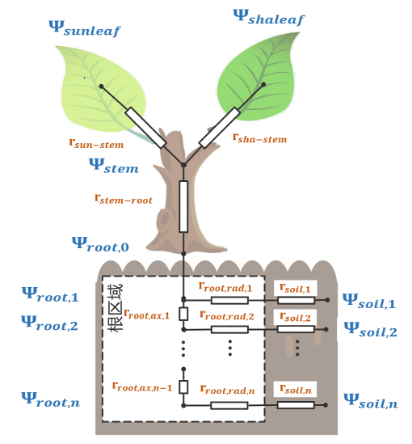
\includegraphics{Figures/植被水力模式/CoLM植物水力模型示意图.png}
\caption{CoLM植物水力模型示意图。}
\label{fig:CoLM植物水力模型示意图}
\end{figure}
}


CoLM植物水势的动态模拟假设植物水分传输为稳恒流,并将其类比为电路问题 
\citep{van1948water},即水分传输速率正比于水势差和水力导度。
地上部分四个节点的水势由Darcy定律表达,满足以下方程:
\begin{equation}\label{q_sunstem}
q_{ {sun \leftarrow stem }}=k_{{sun} \leftarrow  {stem}}\left(\Psi_{sunleaf}-\Psi_{stem}\right)
\end{equation}
\begin{equation}
q_{ {sha \leftarrow stem }}=k_{ {sha} \leftarrow {stem}}\left(\Psi_{shaleaf}-\Psi_{ {stem }}\right)
\end{equation}
\begin{equation}
q_{ {stem \leftarrow root }}=k_{ {stem } \leftarrow  { root }}\left(\Psi_{ {stem }}-\Psi_{ {root }, 0}\right)
\end{equation}
$k_{sun \leftarrow stem}$,$k_{sha \leftarrow stem }$,$k_{stem \leftarrow root }$ 分别代表茎到阳叶的水力导度、茎到阴叶的水力导度和根到茎的水力导度。
水力导度随水势降低而降低,是关于茎和根水势的函数 (详见章节 \ref{植物水力导度的衰减}) 。地表根水势$\Psi_{root,0}$是关于每层土壤水势 ($\Psi_{soil,i}$) 
及根总吸水速率 ($q_{root,0}$) 的函数,由地下植物水力过程所计算 (详见章节 \ref{地下植物水力过程}):
\begin{equation}\label{Psi_root_0}
\Psi_{root, 0}=R\left(\Psi_{ {soil }, i}, q_{root, 0}\right)
\end{equation}
$q_{sun \leftarrow stem}$,$q_{sha \leftarrow stem }$,$q_{stem \leftarrow root }$分别代表茎到阳叶的水流速、茎到阴叶的水流速和根到茎的水流速。
水流速在各节点由于稳恒流假设,满足水分守恒方程:
\begin{equation}
E_{sun}=q_{sun \leftarrow  stem}
\end{equation}
\begin{equation}
E_{ {sha }}=q_{ sha \leftarrow stem}
\end{equation}
\begin{equation}
q_{ {sun \leftarrow stem }}+q_{ {sha \leftarrow stem }}=q_{ {stem \leftarrow root }}
\end{equation}
\begin{equation}\label{q_stemroot}
q_{stem \leftarrow root}=q_{root, 0}
\end{equation}
$E_{sun}$代表阳叶蒸腾速率,$E_{sha}$代表阴叶蒸腾速率。它们是由无水分胁迫情况下的叶片蒸腾 ($E_{sun,max}$, $E_{sha,max}$) 
和受叶片水势 ($\Psi_{sunleaf}$,$\Psi_{shaleaf}$) 控制的蒸腾衰减函数所组成(详见章节 \ref{植物水力导度的衰减})。
同时,无水分胁迫的叶片蒸腾是在最大气孔导度 ($g_{s,sun,max}$, $g_{s,sha,max}$) 的条件下,
运用章节 \ref{一维植被湍流交换模型} 植被覆盖地表湍流通量的计算方案所推导得出。最大气孔导度的计算则需要植物水力模式、光合作用模式、气孔导度模式耦合解出 (详见章节 \ref{气体扩散方程和气孔导度模型})。

\section{植物水力导度的衰减}\label{植物水力导度的衰减}
植物水势下降导致的空穴现象会严重降低水分在植物内部的传导能力。我们将实验上观测到水力导度随水势变化的S型脆弱性曲线 
\citep{sperry1988method,gentine2016allometry,neufeld1992genotypic,pammenter1998mathematical,plaut2012hydraulic}
 引入到模型,对植物水力栓塞进行参数化,得到节点间的水力导度$k_{i\gets j}$ (从节点$j$到$i$的传输):
\begin{equation}
k_{i \leftarrow j}=k_{\max } \cdot 2^{-\left(\frac{\Psi_{\mathbf{j}}}{p 50}\right)^{c_{k}}}
\end{equation}
其中$k_{max}$表示最大水力导度 (\unit{s^{-1}})。$\Psi_j$代表节点$j$的水势 (\unit{mm.H_2O}),$p50$代表水力导度降低 50\% 时的水势 (\unit{mm.H_2O}),$c_k$代表脆弱性曲线的形状参数。


实验数据发现气孔导度和叶片水势同样存在S型曲线关系 \citep{klein2014variability},
CoLM植物水力模式引入蒸腾速率随叶片水势 ($\Psi_{sunleaf}$,$\Psi_{shaleaf}$)的衰减函数 \citep{kennedy2019implementing}:
\begin{equation}\label{e_sun_a}
E_{ {sun }}=E_{ {sun,max }} \cdot 2^{-\left(\frac{\Psi_{ {sunleaf }}}{p 50}\right)^{c_{k}}}
\end{equation}
\begin{equation}\label{e_sha_a}
E_{ {sha }}=E_{ {sha,max }} \cdot 2^{-\left(\frac{\Psi_{ {shaleaf }}}{p 50}\right)^{c_{k}}}
\end{equation}
$E_{sun,max} $和$E_{sha,max}$分别表示无水分胁迫情况下的阳叶、阴叶的最大蒸腾速率。

\section{地下植物水力过程}\label{地下植物水力过程}
水力重分配是重要的植物地下水力过程,它描述了水分通过地下根系从湿润土壤层向干燥土壤层的传输。
它被认为是一个被动的受水势梯度所驱动的水分传输过程。基于该物理原理,Amenu水力重分配模型 \citep{amenu2008}被CoLM采用 \citep{zhu2017incorporating},
并与土壤水文过程和植被地上水力过程相耦合 \citep{li2021new},考虑包括在根、茎和叶等地上节点外的, 
$n$个代表不同土壤深度的根系水力节点和$n$个土壤水力节点 (如图~\ref{fig:CoLM植物水力模型示意图})。模式中的水力传导包括轴向水力传导和径向水力传导。
轴向水力传导由Darcy定律所表示:
\begin{equation}\label{k_axi}
k_{ax,i}\left(\Psi_{r,i}-\Psi_{r,i+1}\right)=q_{ax,i}
\end{equation}
其中$k_{ax,i}$代表第$i+1$层到第i层根节点间的轴向水力导度,$q_{ax,i}$代表相应的轴向水分传输速率,
$\Psi_{r,i}$代表第$i$层根节点的水势。$i$取值1到$n-1$,$n$代表土壤总层数。\\
径向水力传导方程:
\begin{equation}\label{k_radi}
k_{rad,i}\left(\Psi_{soil,i}-\Psi_{r,i}\right)=q_{rad,i}
\end{equation}
其中$k_{rad,i}$代表第$i$层土壤节点到根节点间的径向水力导度,
$q_{rad,i}$代表相应的径向水分传输速率,$\Psi_{soil,i}$代表第$i$层土壤节点的水势,$i$取值1到$n$。



对于第2到$n$层的土壤根节点存在水分平衡方程:
\begin{equation}\label{q_axi}
q_{a x, i}+q_{r a d, i}=q_{a x, i-1}
\end{equation}
其中$i=2, \ldots, n$,方程~\eqref{q_axi} 实际上是$n-1$个方程组。


另外,由表层根节点的水分平衡方程可得:
\begin{equation}\label{q_ax1}
q_{ax,1}+q_{rad, 1}=q_{root,0}
\end{equation}
将方程(\ref{k_axi})和(\ref{k_radi})代入(\ref{q_axi})和(\ref{q_ax1}),则得到关于$ \Psi_{r,i}$的$n$个线性方程组。
这$n$个线性方程组描述了在植物地下水力过程作用下,根水势垂直分布。其输入包括土壤水势垂直分布 ($\Psi_{soil,i}$) 和根总吸水速率 ($q_{root,0}$)。
其输出包括根水势垂直分布 ($\Psi_{r,i}$) 和根吸水速率垂直分布 ($q_{rad,i}$)。因此,地下植物水力过程可以被简化地表示为公式(\ref{Psi_root_0})。

\section{气孔导度的水分胁迫}\label{气孔导度的水分胁迫}
土壤水分亏缺对植物生理的影响被表现在水分胁迫因子上,水分胁迫因子作为取值 $0\sim 1$ 的无量纲变量,作用在光合作用各限制因子上,见公式(\ref{V_cmax_a})--(\ref{R_d1})。

植物水力模式未开启时,水分胁迫因子 ($\beta$) 决定于根的垂直分布比例和土壤水势,其计算不区分阴叶和阳叶:
\begin{equation}\label{beta_0}
\beta=\sum_{i=1}^{n} froot_i \beta_{i}
\end{equation}

\begin{equation}\label{beta_i}
\beta_{i}=\frac{\Psi_{\max }-\Psi i}{\Psi_{\max }-\Psi_{s a t}}
\end{equation}
$froot_i$是第i层的根含量,$\beta_i$是第$i$层的水分胁迫因子;它根据每层土壤的实际水势 (${\Psi}_i$),最大水势 (${\Psi}_{max}$)和饱和水势 (${\Psi}_{sat}$)计算得出。

当植物水力模式开启时,水分胁迫对植被的直接影响是植物水势的降低,气孔通过关闭以尽量保持植物的导水能力,但同时也导致叶片光合速率降低。
植物水力模式符合植物生理学理论和物理规律,水分胁迫因子 ($\beta_{sun}$,$\beta_{sha}$) 决定于气孔导度的衰减比例,其计算区分阳叶和阴叶:
\begin{equation}\label{beta_sun}
\beta_{sun}=g_{s,sun} / g_{s,sun,max }
\end{equation}
\begin{equation}\label{beta_sha}
\beta_{sha}=g_{s,sha} / g_{s,sha, \max }
\end{equation}
$g_{s,sun}$和$g_{s,sun}$分别代表阳叶和阴叶的实际气孔导度,
$g_{s,sun,max}$和$g_{s,sun,max}$分别代表阳叶和阴叶在无水分胁迫条件下的最大气孔导度。
水分胁迫的求解需要耦合地表冠层湍流参数化方案和光合气孔模式。


最大气孔导度 ($g_{s,sun,max}$和$g_{s,sun,max}$) 的计算依赖于光合气孔模式。
光合气孔模式中,气孔导度为方程(\ref{ei_cs})的正根,(\ref{ei_cs})和(\ref{ci_1})联立可表示为实际气孔导度关于净光合作用速率的隐式方程:
\begin{equation}\label{gs_0}
g_{s}=g\left(A_{n}\right)
\end{equation}
由于水分胁迫是光合作用中的相关参数,公式(\ref{gs_0})可以写成:
\begin{equation}\label{gs_1}
g_{s}=g\left(f_{photo}(\beta)\right)
\end{equation}
最大气孔导度可表述为:
\begin{equation}\label{gs_sunmax}
g_{s,  { sun,max }}=\frac{g\left(f_{ {photo }}\left(\beta_{ {sun }}\right)\right)}{\beta_{ {sun }}}
\end{equation}
\begin{equation}\label{gs_shamax}
g_{s, sha, \max }=\frac{g\left(f_{photo}\left(\beta_{s h a}\right)\right)}{\beta_{s h a}}
\end{equation}
$f_{photo}$代表公式(\ref{An1})的光合作用模型。


最大气孔导度一方面是植物水力模式水分胁迫计算的必要变量(公式(\ref{beta_sun})和(\ref{beta_sun})),
另一方面,为地表冠层湍流参数化方案中叶片最大蒸腾速率计算提供重要输入 (如图~\ref{fig:光合气孔模式和植物水力模式的耦合示意图})。
地表冠层湍流参数化方案中的叶片最大蒸腾速率$(E_{sun,max}$和$E_{sha,max}$) 可简化地表示为:
\begin{equation}\label{E_sunmax}
E_{sun, \max }=E\left(g_{s, sun, \max }\right)
\end{equation}
\begin{equation}\label{E_shamax}
E_{sha, \max }=E\left(g_{s, sha, \max }\right)
\end{equation}
其中,与植物水力模式无关的参数、变量在此省略,完整表述见植被覆盖地表湍流通量的计算方案 (见章节 \ref{一维植被湍流交换模型})。


实际气孔导度 ($g_{s,sun}$和$g_{s,sun}$) 的计算同样依赖于地表冠层湍流参数化方案。由于植物水力模式可以求解植物叶片实际蒸腾 ($E_{sun}$和$E_{sha}$),
可以利用公式(\ref{E_sunmax})和(\ref{E_shamax})的逆函数求解气孔导度:
\begin{equation}\label{g_ssun}
g_{s, s u n}=E^{-1}\left(E_{s u n}\right)
\end{equation}
\begin{equation}\label{g_ssha}
g_{s, sha}=E^{-1}\left(E_{s h a}\right)
\end{equation}
耦合植物水力模式、光合气孔模式和地表冠层湍流参数化方案,再利用公式(\ref{beta_sun})和(\ref{beta_sha})可以完整地求解植物水力模式下的植物水分胁迫 (如图 \ref{fig:光合气孔模式和植物水力模式的耦合示意图})。
{
    \begin{figure}[]
    \centering
    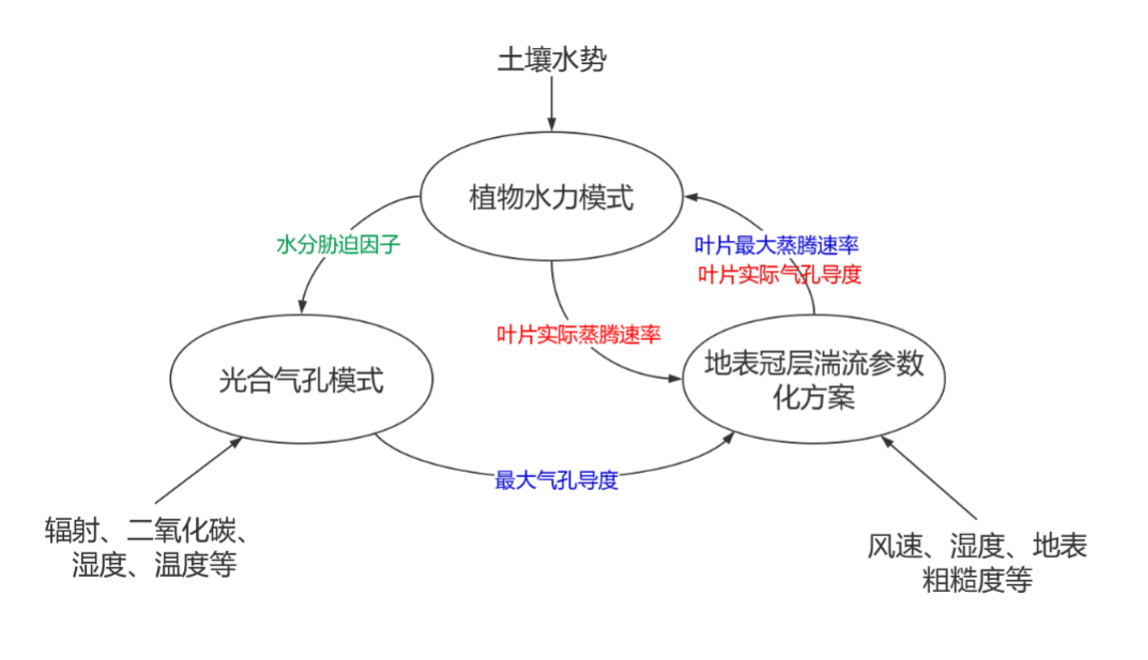
\includegraphics{Figures/植被水力模式/光合气孔模式和植物水力模式的耦合示意图.png}
    \caption{光合气孔模式和植物水力模式的耦合示意图。}
    \label{fig:光合气孔模式和植物水力模式的耦合示意图}
    \end{figure}
    }
    
\section{数值计算方案}\label{数值计算方案}
求解植物水势、水分胁迫、气孔导度和叶片蒸腾速率,需要耦合植物水力模式、光合气孔模式和地表冠层参数化方案。
耦合描述植物水势变化的动力方程组(公式(\ref{q_sunstem})--(\ref{q_stemroot}), (\ref{e_sun_a}) 和(\ref{e_sha_a})),
地表冠层参数化方案 (公式(\ref{E_sunmax})--(\ref{g_ssha})),
光合气孔模式的最大气孔导度计算 (公式(\ref{gs_sunmax})和(\ref{gs_shamax})), 植物水分胁迫计算(公式(\ref{beta_sun})和(\ref{beta_sha})),共18个方程,
求解包括4个植物地上水势节点 ($\Psi_{sunleaf}$, $\Psi_{shaleaf}$, $\Psi_{stem}$和$\Psi_{root,0}$),8个水分传输速率 
($q_{sun-stem}$,$q_{sha-stem}$,$q_{stem-root}$,$q_{root,0}$,$E_{sun}$,$E_{sun,max}$和$E_{sun,max}$) ,4个气孔导度变量
 ($g_{s,sun}$,$g_{s,sun}$,$g_{s,sun,max}$,$g_{s,sun,max}$),2个水分胁迫变量 ($\beta_{sun}$,$\beta_{sha}$) 在内的共18个未知量。

然而,由于以上18个方程中存在隐形方程,我们求解该问题时,引入三重嵌套数值求解办法。其主要步骤如下(图 \ref{fig:植物水力模式的数值模拟流程图}):
\begin{enumerate}
    \item 利用冠层模型,计算叶片温度 ($T_{l,sun}$,$T_{l,sha}$);
    \item 利用光合气孔模式,计算最大气孔导度 ($g_{s,sun,max}$和$g_{s,sun,max}$);
    \item 根据最大气孔导度,计算叶片最大蒸腾速率 ($E_{sun,max}$和$E_{sun,max}$);
    \item 将叶片最大蒸腾速率输入植物水力模式,计算水分胁迫 ($\beta_{sun}$,$\beta_{sha}$);
    \item 更新光合气孔模式的水分胁迫,迭代计算,判断胞间二氧化碳浓度是否收敛,若收敛,进入第 (6) 步;若不收敛,重复此步骤;
    \item 更新气孔导度,判断阴叶、阳叶水分胁迫是否收敛,若收敛,进入第 (7) 步,若不收敛,回到第 (2) 步;
    \item 更新植物水势和叶片蒸腾,判断叶片温度是否收敛,若收敛,植物水力模式求解完成,若不收敛,回到第 (1) 步。
\end{enumerate}

气孔导度详细迭代

{
    \begin{figure}[]
    \centering
    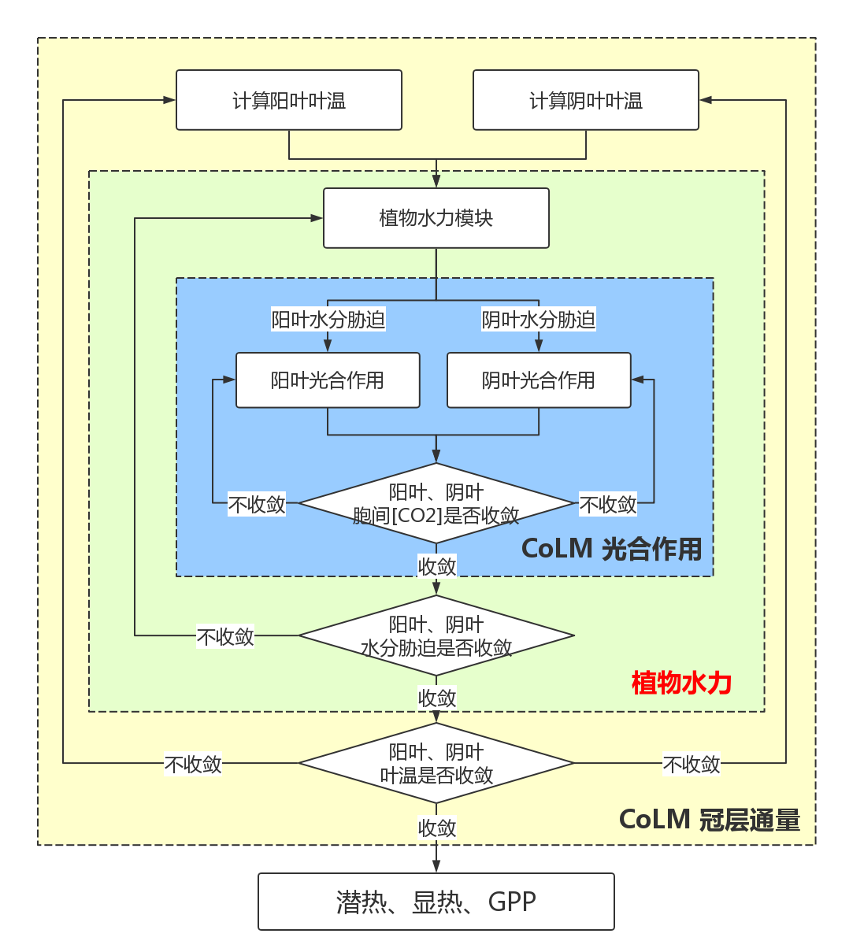
\includegraphics{Figures/植被水力模式/植物水力模式的数值模拟流程图.png}
    \caption{植物水力模式的数值模拟流程图。}
    \label{fig:植物水力模式的数值模拟流程图}
    \end{figure}
    }

